\chapter{Study design}

The used method of the study design is called The One-Group Pretest-Posttest Design. This enable to compare the situation before and after treatment within each subject like shown in figure \ref{fig:design1}. \cite{gottman1969}
\begin{figure}[H]
	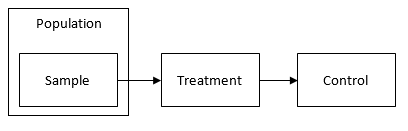
\includegraphics[width=0.4\textwidth]{figures/inseries1}
	\caption{The procedure of studies with The One-Group Pretest-Posttest Design.}
	\label{fig:design1}
\end{figure}

Within this study the arms of the subjects will be cuffed. To avoid any carry-over effect, the measurements under normal conditions will be done first. As shown in figure \ref{fig:design2} that means beginning with the control and then the treatment, which is in this case a partial occlusion of the blood flow.
\begin{figure}[H]
	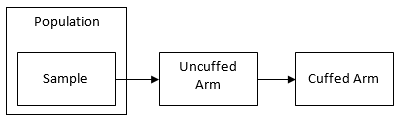
\includegraphics[width=0.4\textwidth]{figures/inseries2}
	\caption{The procedure of this study with The One-Group Pretest-Posttest Design.}
	\label{fig:design2}
\end{figure}